% Provenance (never printed): see sources/outline_sources.md (Year 3: rift
% models, normal-fault systems, metamorphic core complexes, strike-slip
% systems). Brief: sources/book5/BRIEFS.md, ch. 9. Curves from
% figdata/bachelor-3/domino_extension.py and rollover.py. Exercise and problem
% values in the Book 5 scratch calculator calc/ch09.py.
\chapter{Extensional and Strike-Slip Tectonics}\label{ch:b3:extension-strike-slip}

Between the Sierra Nevada and the Colorado Plateau, ranges and basins
alternate like the furrows of a field, each range a block of crust tilted
along a normal fault. In the cores of some of these ranges, rocks that were
buried 23 to \qty{30}{km} deep, at 500 to \qty{650}{\celsius}, now lie at the
surface, under a single fault that dips only a few degrees. A continent can
be pulled apart by a factor of two or more, and torn sideways along faults
that bend, step and open basins as deep as \qty{10}{km}. This chapter builds
the geometry of extension and of strike-slip faulting, the few rules that
govern it, and the evidence that real systems leave.
% ledger: cooper10:snake-range, mcq05:basin-range, tb93:dead-sea-basin

\begin{recall}
Normal, strike-slip and transform faults, the half-graben and the continental
rift are in the Year 1 volume, in its chapters on rifts and on faults, folds
and fabrics, with Anderson's theory: with $\sigma_1$ vertical, normal faults
dip $\ang{45} + \phi/2$, about \ang{60}; with $\sigma_2$ vertical, strike-slip
faults strike at $\ang{45} - \phi/2$ from $\sigma_1$. Byerlee's law of rock
friction, $\tau = 0.85\,\sigma_n$ below \qty{200}{MPa} and $\tau =
\qty{50}{MPa} + 0.6\,\sigma_n$ above, is in its chapter on stress, strain and
rheology. The stretching model, in which the lithosphere is thinned uniformly
by a factor $\beta$, and the rift basin are in the Year 2 volume, in its
chapter comparing sedimentary basins. \omterm{def:b3:deformation-mechanisms:shear-zone}{Shear zones} and mylonites are in
\cref{ch:b3:deformation-mechanisms}; the depth to detachment from an excess
area, $A = Sh$, in \cref{ch:b3:structural-analysis}.
\end{recall}
% ledger: byerlee:1975

\section{Two models of a rift}\label{sec:b3:extension-strike-slip:models}

The stretching model of the Year 2 volume thins the whole lithosphere by the
same factor beneath the same place: crust and mantle thin together,
symmetrically, by pure shear. Many rifted margins are not symmetric: one side
is a wide region of tilted blocks, the other a narrow steep slope, and the
thinning of the mantle lies beside, not beneath, the thinning of the crust.

\begin{definition}[Simple-shear rift model]\label{def:b3:extension-strike-slip:rift-models}
In the \emph{simple-shear rift model}\index{simple-shear rift model} the
lithosphere is pulled apart along a low-angle \omterm{def:b3:deformation-mechanisms:shear-zone}{shear zone} that cuts through it
from the surface to its base. The plate above the \omterm{def:b3:deformation-mechanisms:shear-zone}{shear zone}, the upper
plate, loses its lower part; the plate below, the lower plate, is pulled out
from under it. The thinning of the crust and the thinning of the mantle are
offset sideways, and the two conjugate margins that form when the continent
breaks are asymmetric.
\end{definition}

Real rifts mix the two: brittle faulting in the upper crust, ductile thinning
below, and a mantle that may thin over a wider or a narrower region than the
crust (depth-dependent stretching). Where the hot mantle rises beneath the
rift, or beneath its flank in the simple-shear case, buoyancy raises the
shoulders of the rift, which stand as mountains above the basin floor.

\begin{omfigure}
\begin{tikzpicture}[scale=0.95, >=stealth]
% (a) pure shear
\begin{scope}
\fill[omLithBasalt!40] (0,-3.2) rectangle (6.6,-1.3);
\fill[omLithGranite!50] (0,0) -- (2.2,0) -- (2.5,-0.35) -- (4.1,-0.35) -- (4.4,0) -- (6.6,0) -- (6.6,-1.3)
  -- (4.4,-1.3) -- (3.3,-0.95) -- (2.2,-1.3) -- (0,-1.3) -- cycle;
\fill[omLithBasalt!40] (2.2,-1.3) -- (3.3,-0.95) -- (4.4,-1.3) -- cycle;
\fill[orange!25] (0,-3.2) -- (1.8,-3.2) -- (3.3,-2.1) -- (4.8,-3.2) -- (6.6,-3.2) -- (6.6,-3.7) -- (0,-3.7) -- cycle;
\draw (0,0) -- (2.2,0) -- (2.5,-0.35) -- (4.1,-0.35) -- (4.4,0) -- (6.6,0);
\draw (0,-1.3) -- (2.2,-1.3) -- (3.3,-0.95) -- (4.4,-1.3) -- (6.6,-1.3);
\draw (0,-3.2) -- (1.8,-3.2) -- (3.3,-2.1) -- (4.8,-3.2) -- (6.6,-3.2);
\draw[thick] (2.2,0) -- (2.75,-0.85); \draw[thick] (4.4,0) -- (3.85,-0.85);
\node[font=\scriptsize] at (0.7,-0.65) {crust};
\node[font=\scriptsize, align=center] at (0.9,-2.25) {mantle\\ lithosphere};
\node[font=\scriptsize] at (1.2,-3.48) {asthenosphere};
\draw[<-] (-0.1,0.25) -- (0.6,0.25); \draw[->] (6.0,0.25) -- (6.7,0.25);
\node[font=\small] at (3.3,-4.2) {(a) pure shear};
\end{scope}
% (b) simple shear: crust thinned near the breakaway (left), mantle beneath the upper plate (right)
\begin{scope}[xshift=7.4cm]
\fill[omLithBasalt!40] (0,-3.2) rectangle (6.6,-1.3);
\fill[omLithGranite!50] (0,0) -- (0.9,0) -- (1.2,-0.3) -- (2.2,-0.3) -- (2.5,0) -- (4.0,0)
  .. controls (4.6,0.18) and (5.2,0.18) .. (5.8,0) -- (6.6,0) -- (6.6,-1.3)
  -- (2.9,-1.3) -- (2.0,-0.7) -- (1.2,-1.3) -- (0,-1.3) -- cycle;
\fill[omLithBasalt!40] (1.2,-1.3) -- (2.0,-0.7) -- (2.9,-1.3) -- cycle;
\fill[orange!25] (0,-3.2) -- (3.4,-3.2) -- (4.8,-2.1) -- (6.0,-3.2) -- (6.6,-3.2) -- (6.6,-3.7) -- (0,-3.7) -- cycle;
\draw (0,0) -- (0.9,0) -- (1.2,-0.3) -- (2.2,-0.3) -- (2.5,0) -- (4.0,0)
  .. controls (4.6,0.18) and (5.2,0.18) .. (5.8,0) -- (6.6,0);
\draw (0,-1.3) -- (1.2,-1.3) -- (2.0,-0.7) -- (2.9,-1.3) -- (6.6,-1.3);
\draw (0,-3.2) -- (3.4,-3.2) -- (4.8,-2.1) -- (6.0,-3.2) -- (6.6,-3.2);
\draw[omThm, very thick] (0.9,0) .. controls (2.4,-0.9) and (3.9,-1.8) .. (5.4,-3.2);
\node[font=\scriptsize, align=center] at (5.0,-0.6) {upper plate};
\node[font=\scriptsize, align=center] at (1.3,-2.3) {lower plate};
\node[omThm, font=\scriptsize, align=center] at (3.0,-2.15) {shear\\ zone};
\node[font=\scriptsize, align=center] at (4.9,0.42) {uplifted flank};
\draw[<-] (-0.1,0.25) -- (0.6,0.25); \draw[->] (6.0,0.25) -- (6.7,0.25);
\node[font=\small] at (3.3,-4.2) {(b) simple shear};
\end{scope}
\end{tikzpicture}

\par\smallskip{\small Two end-member models of a rift (not to scale). (a) Pure
shear: crust and mantle lithosphere thin together beneath the rift, with
normal faults on both sides. (b) Simple shear: a low-angle \omterm{def:b3:deformation-mechanisms:shear-zone}{shear zone} crosses
the lithosphere; the crust thins near its surface trace, the mantle beneath
the far side, under the upper plate, so that the rift is asymmetric and its
flank above the thinned mantle is uplifted.}\label{fig:b3:extension-strike-slip:models}
\end{omfigure}

\section{Normal-fault systems}\label{sec:b3:extension-strike-slip:faults}

\begin{definition}[Domino faulting]\label{def:b3:extension-strike-slip:domino}
In \emph{domino faulting}\index{domino faulting} a set of parallel planar
normal faults cuts the upper crust into rigid blocks which, as the region
extends, rotate together like a row of books falling over: the faults become
less steep and the beds, first horizontal, tilt the other way.
\end{definition}

\begin{theorem}[Extension by dominoes]\label{thm:b3:extension-strike-slip:domino}
Let rigid blocks bounded by parallel planar faults that first dipped
$\theta_0$ rotate until the faults dip $\theta$. The beds then dip $\theta_0
- \theta$, away from the faults, and the region has been extended by the
factor
\[
  \beta = \frac{\sin\theta_0}{\sin\theta} .
\]
\end{theorem}

\begin{proof}
The blocks are rigid, so the perpendicular distance $d$ between two
neighbouring faults does not change. Along a horizontal line, two parallel
planes that dip $\theta$ and are $d$ apart cut a segment of length $d/\sin
\theta$; the region's width scales as the length of that segment, from
$d/\sin\theta_0$ to $d/\sin\theta$. The blocks turn through the angle by
which the faults have flattened, $\theta_0 - \theta$, and the beds, horizontal
at first, turn with them.
\end{proof}

Rotation alone gives modest extension: faults that start at \ang{60} and
flatten to \ang{30} extend the region by $\beta = 1.73$. They cannot rotate
for ever: a fault becomes harder to slip as it flattens, because the vertical
$\sigma_1$ presses on it more and shears it less.

\begin{proposition}[Frictional lock-up of a normal fault]\label{prop:b3:extension-strike-slip:lockup}
Let a cohesionless fault with the friction coefficient $\mu$ make the angle
$t$ with $\sigma_1$, all stresses effective. It slips when the ratio of the
principal stresses reaches
\[
  \frac{\sigma_1}{\sigma_3} = \frac{1 + \mu\cot t}{1 - \mu\tan t} ,
\]
which is least, $(\sqrt{1 + \mu^2} + \mu)^2$, at $\tan2t = 1/\mu$, and
infinite at $\tan t = 1/\mu$. With $\sigma_1$ vertical, the fault's dip is
$\ang{90} - t$: a normal fault dipping less than $\arctan\mu$ cannot slip at
all.
\end{proposition}

\begin{proof}
Write $m = (\sigma_1 + \sigma_3)/2$ and $s = (\sigma_1 - \sigma_3)/2$. On
the plane, $\sigma_n = \sigma_1\sin^2t + \sigma_3\cos^2t = m - s\cos2t$ and
$\tau = (\sigma_1 - \sigma_3)\sin t\cos t = s\sin2t$. Slip needs $\tau =
\mu\sigma_n$; dividing by $\sigma_3\sin t\cos t$ and collecting $\sigma_1$
gives the ratio, whose denominator vanishes at $\tan t = 1/\mu$. In the other
form the condition reads $s(\sin2t + \mu\cos2t) = \mu m$. The bracket is at
most $\sqrt{1 + \mu^2}$, reached at $\tan2t = 1/\mu$, where slip needs the
least $s/m = \mu/\sqrt{1 + \mu^2}$; then $\sigma_1/\sigma_3 = (m + s)/(m - s) =
(\sqrt{1 + \mu^2} + \mu)/(\sqrt{1 + \mu^2} - \mu) = (\sqrt{1 + \mu^2} +
\mu)^2$, since the product of the last two brackets is 1.
\end{proof}

With Byerlee's $\mu = 0.6$, the best-oriented normal fault dips \ang{60.5} and
slips when $\sigma_1 = 3.12\,\sigma_3$, a fault at \ang{45} needs $4.0$, and
none dipping less than \ang{31} slips; with $\mu = 0.85$ the lock-up dip is
\ang{40}. The figure below shows both results. When a set of dominoes nears
lock-up, a new set of steep faults cuts the old one: highly extended regions
show several generations of faults.

\begin{omfigure}
\begin{tikzpicture}
\begin{groupplot}[group style={group size=2 by 1, horizontal sep=1.6cm},
  omrecord, width=0.47\linewidth, height=0.42\linewidth, title style={font=\small},
  legend style={font=\scriptsize, legend cell align=left}]
\nextgroupplot[title={(a) extension by rigid dominoes}, xlabel={present fault dip $\theta$ (\unit{\degree})},
  ylabel={extension factor $\beta$}, xmin=10, xmax=70, ymin=1, ymax=4,
  legend style={at={(0.97,0.97)}, anchor=north east}]
% computed in figdata/bachelor-3/domino_extension.py
\addplot[omDef, thick] table[x=dip, y=b70] {figdata/out/bachelor-3-domino_extension-beta.dat};
\addlegendentry{$\theta_0 = \ang{70}$}
\addplot[red!70!black, thick, densely dashed] table[x=dip, y=b60] {figdata/out/bachelor-3-domino_extension-beta.dat};
\addlegendentry{$\theta_0 = \ang{60}$}
\addplot[black, thick, densely dotted] table[x=dip, y=b45] {figdata/out/bachelor-3-domino_extension-beta.dat};
\addlegendentry{$\theta_0 = \ang{45}$}
\nextgroupplot[title={(b) stress ratio needed for slip}, xlabel={fault dip (\unit{\degree})},
  ylabel={$\sigma_1/\sigma_3$}, xmin=20, xmax=90, ymode=log, ymin=1, ymax=40,
  log ticks with fixed point, ytick={1,2,5,10,20,40},
  legend style={at={(0.97,0.97)}, anchor=north east}]
\addplot[omDef, thick] table[x=dip, y=r060] {figdata/out/bachelor-3-domino_extension-lockup.dat};
\addlegendentry{$\mu = 0.6$}
\addplot[red!70!black, thick, densely dashed] table[x=dip, y=r085] {figdata/out/bachelor-3-domino_extension-lockup.dat};
\addlegendentry{$\mu = 0.85$}
\end{groupplot}
\end{tikzpicture}

\par\smallskip{\small (a) Extension factor of a domain of rigid dominoes as
its faults rotate from the initial dip $\theta_0$ to $\theta$. (b) Ratio of
the effective principal stresses needed to slip a normal fault of a given dip
under a vertical $\sigma_1$, for Byerlee's two friction coefficients: least
near \ang{60} and \ang{65}, infinite at the lock-up dips \ang{31} and
\ang{40}.}\label{fig:b3:extension-strike-slip:domino}
\end{omfigure}

Many large normal faults are curved, steep at the surface and flattening at
depth into a nearly horizontal fault or \omterm{def:b3:deformation-mechanisms:shear-zone}{shear zone}.

\begin{definition}[Detachment fault, listric fault, rollover anticline]\label{def:b3:extension-strike-slip:detachment}
A \emph{detachment fault}\index{detachment fault} is a low-angle normal fault
or \omterm{def:b3:deformation-mechanisms:shear-zone}{shear zone} of large displacement, kilometres to tens of kilometres, that
separates an extended upper plate from a lower plate deformed differently. A
\emph{listric fault}\index{listric fault} is a normal fault whose dip
decreases with depth, its profile concave upward. As the hanging wall of a
listric fault moves down and away, it bends to stay in contact with the
fault: its beds tilt towards the fault in a broad fold, the \emph{rollover
anticline}\index{rollover anticline}.
\end{definition}

\begin{method}[The constant-heave construction]\label{met:b3:extension-strike-slip:heave}
To draw the hanging wall of a \omterm{def:b3:extension-strike-slip:detachment}{listric fault} after a horizontal displacement
$H$, the heave, on a section parallel to the slip:
\begin{enumerate}
  \item Divide the hanging wall into vertical columns. Move each column
        sideways by $H$, away from the footwall.
  \item Lower each column by the fall of the fault beneath it: a column that
        started where the fault lies at the depth $f(x)$ and ends where it
        lies at $f(x + H)$ drops by $f(x + H) - f(x)$, which brings its base
        back onto the fault.
  \item The space left between the footwall and the moved hanging wall is the
        half-graben, filled as it opens by sediments that thicken towards the
        fault.
\end{enumerate}
Read backwards, the construction restores the section and predicts the shape
of the fault from the shape of the rollover.
\end{method}

The area below the original level of a bed, counted from the fault, is
the area of \cref{ch:b3:structural-analysis} with the sign changed: $A =
H(D - z_0)$ for a bed first at the depth $z_0$ above a detachment at the
depth $D$, since the rock under the bed keeps its area while its length grows
by $H$. Measuring $A$ and $H$ on a seismic section gives the depth of the
detachment. The figure below draws the construction.

\begin{omfigure}
\begin{tikzpicture}
\begin{axis}[width=0.9\linewidth, height=0.36\linewidth, omsection,
  xmin=-2, xmax=24, ymin=0, ymax=6, y dir=reverse,
  xlabel={distance (\unit{km})}, ylabel={depth (\unit{km})},
  legend style={font=\scriptsize, legend cell align=left, at={(0.98,0.27)}, anchor=south east}]
% computed in figdata/bachelor-3/rollover.py (heave 2 km, detachment at 5 km)
\addplot[name path=fault, black, very thick] table[x=x, y=z] {figdata/out/bachelor-3-rollover-fault.dat};
\addlegendentry{listric fault}
\addplot[name path=top, omDef, thick] table[x=x, y=z] {figdata/out/bachelor-3-rollover-top.dat};
\addlegendentry{top of the hanging wall}
\addplot[omDef, thick, densely dashed] table[x=x, y=z] {figdata/out/bachelor-3-rollover-bed.dat};
\addlegendentry{a bed first at \qty{2}{km}}
\addplot[gray, dashed, forget plot] coordinates {(-2,0) (24,0)};
\addplot[gray, dashed, forget plot] coordinates {(-2,5) (24,5)};
\node[font=\scriptsize, anchor=west] at (axis cs:15,5.35) {detachment};
\node[font=\scriptsize] at (axis cs:3.9,0.45) {half-graben};
\node[font=\scriptsize] at (axis cs:-1,1.5) {footwall};
\node[font=\scriptsize] at (axis cs:9.5,1.15) {rollover};
\end{axis}
\end{tikzpicture}

\par\smallskip{\small A \omterm{def:b3:extension-strike-slip:detachment}{listric fault} dipping \ang{60} at the surface and
flattening into a detachment at \qty{5}{km}, after a heave of \qty{2}{km}
drawn by the constant-heave construction. The top of the hanging wall and a
deeper bed sag towards the fault in a rollover; the area below the original
top, \qty{10}{km^2}, is the heave times the depth of the detachment, and below
the deeper bed \qty{6}{km^2}, the heave times its height above it.}\label{fig:b3:extension-strike-slip:rollover}
\end{omfigure}

Normal faults are not endless. Where one fault dies out along strike, its
displacement passes to another, often dipping the other way, and the
half-grabens of a rift alternate in polarity along its length.

\begin{definition}[Transfer zone]\label{def:b3:extension-strike-slip:transfer}
A \emph{transfer zone}\index{transfer zone} is the region between two
overlapping or offset normal-fault segments, or rift segments, across which
the extension passes from one to the other: a relay ramp between two faults
of the same polarity, a high between half-grabens of opposite polarity, or a
strike-slip fault, the transfer fault, parallel to the extension.
\end{definition}

\section{Metamorphic core complexes}\label{sec:b3:extension-strike-slip:core}

\begin{definition}[Metamorphic core complex, rolling hinge]\label{def:b3:extension-strike-slip:core-complex}
A \emph{metamorphic core complex}\index{metamorphic core complex} is a dome of
metamorphic rocks and mylonites, brought up from the middle or lower crust,
beneath a \omterm{def:b3:extension-strike-slip:detachment}{detachment fault} whose upper plate is a mosaic of tilted blocks of
upper-crustal rocks. In the \emph{rolling hinge}\index{rolling hinge} model,
the detachment slips at a moderate dip at depth; as the upper plate moves
away, the unloaded footwall rises by isostasy and bends, so that each part of
the fault rotates to a low dip, and stops slipping, once it has passed through
a hinge that migrates with the extension.
\end{definition}

The mylonites of the footwall record the deep part of the story: they are
the \omterm{def:b3:deformation-mechanisms:shear-zone}{shear zone} of \cref{ch:b3:deformation-mechanisms}, and their \omterm{def:b3:deformation-mechanisms:kinematic}{kinematic
indicators} give the sense of transport of the upper plate. Higher up, the
same rocks pass through the brittle--ductile transition and are overprinted by
cataclasites and breccias just beneath the fault. In the northern Snake Range
of Nevada, garnet-bearing schists of the footwall reached 6 to \qty{8}{kbar}
and 500 to \qty{650}{\celsius}, burial depths of 23 to \qty{30}{km}; the
detachment that brought them up is interpreted as a \omterm{def:b3:extension-strike-slip:core-complex}{rolling hinge}.
% ledger: cooper10:snake-range

\begin{omfigure}
\begin{tikzpicture}[scale=1.0, >=stealth]
% upper plate dominoes on the left
\foreach \x in {0.0,0.9,1.8} {
  \fill[omLithSand] (\x,0) -- (\x+0.8,0) -- (\x+1.3,-0.9+0.25*\x) -- (\x+0.4,-1.5+0.2*\x) -- cycle;
  \draw (\x,0) -- (\x+0.8,0) -- (\x+1.3,-0.9+0.25*\x) -- (\x+0.4,-1.5+0.2*\x) -- cycle;
}
\fill[omLithGranite!45] (0,-2.6) -- (0,-1.6) .. controls (2.5,-1.2) and (4.0,-0.15) .. (6.0,-0.1)
  .. controls (8.0,-0.15) and (9.5,-0.9) .. (11.2,-1.0) -- (11.2,-2.6) -- cycle;
\fill[pattern=horizontal lines, pattern color=gray] (0,-1.6) .. controls (2.5,-1.2) and (4.0,-0.15) .. (6.0,-0.1)
  .. controls (8.0,-0.15) and (9.5,-0.9) .. (11.2,-1.0) -- (11.2,-1.35)
  .. controls (9.5,-1.25) and (8.0,-0.5) .. (6.0,-0.45) .. controls (4.0,-0.5) and (2.5,-1.55) .. (0,-1.95) -- cycle;
\draw[omThm, very thick] (0,-1.6) .. controls (2.5,-1.2) and (4.0,-0.15) .. (6.0,-0.1)
  .. controls (8.0,-0.15) and (9.5,-0.9) .. (11.2,-1.0);
% upper plate to the right, still in place
\fill[omLithSand] (8.4,0) -- (11.2,0) -- (11.2,-1.0) .. controls (10.2,-0.95) and (9.3,-0.75) .. (8.4,-0.35) -- cycle;
\draw (8.4,0) -- (11.2,0); \draw (8.4,0) -- (8.4,-0.35);
\node[font=\scriptsize] at (9.9,-0.45) {upper plate};
\node[font=\scriptsize] at (1.5,0.3) {tilted blocks};
\node[omThm, font=\scriptsize] at (6.0,0.15) {detachment};
\node[font=\scriptsize] at (6.0,-0.75) {mylonites};
\node[font=\scriptsize, align=center] at (6.0,-1.8) {middle-crustal\\ footwall};
\draw[->, thick] (6.0,-2.9) -- (6.0,-2.2) node[pos=0, below, font=\scriptsize] {isostatic rise};
\draw[->, omThm] (10.4,0.3) -- (11.1,0.3);
\draw[->, omThm] (1.0,0.55) -- (0.3,0.55);
\draw[dashed] (7.6,-0.3) -- (8.6,-1.5) node[below, font=\scriptsize] {rolling hinge};
\end{tikzpicture}

\par\smallskip{\small Anatomy of a \omterm{def:b3:extension-strike-slip:core-complex}{metamorphic core complex} (not to scale).
The footwall of the detachment, a dome of middle-crustal rocks with a
carapace of mylonites, rises beneath the upper plate as it is pulled away to
both sides; the part of the detachment that has passed the \omterm{def:b3:extension-strike-slip:core-complex}{rolling hinge} has
been bent to a low dip and no longer slips. Tilted blocks of the upper plate
rest on the detachment.}\label{fig:b3:extension-strike-slip:core}
\end{omfigure}

The low dips are a paradox: by the lock-up proposition no normal fault dipping
less than about \ang{31} should slip under a vertical $\sigma_1$ with
Byerlee's friction. The \omterm{def:b3:extension-strike-slip:core-complex}{rolling hinge} is one way out: the active part of the
fault is steeper than what is seen. The others are a fault weakened by clays
or by fluids at high pressure, which lowers the effective $\mu$, or a stress
field rotated near a \omterm{def:b3:deformation-mechanisms:shear-zone}{shear zone} at depth; earthquakes on low-angle normal
faults are rare, which favours slip while steep or slip without earthquakes.

\section{Strike-slip systems}\label{sec:b3:extension-strike-slip:strike-slip}

In clay-cake experiments and in nature, a strike-slip fault does not cut a
clean plane through a cover of sediments: it grows as a band of short,
en-echelon fractures with consistent angles.

\begin{definition}[Riedel shear]\label{def:b3:extension-strike-slip:riedel}
In a zone of strike-slip simple shear, \emph{Riedel shears}\index{Riedel shear}
are the short shear fractures that form first, in two sets: the R
shears, at a small angle to the zone and with its sense of slip, and the R$'$
shears, at a large angle and with the opposite sense. Later P shears, symmetric
to the R shears about the zone, and tension fractures T complete the pattern.
\end{definition}

\begin{proposition}[Riedel angles]\label{prop:b3:extension-strike-slip:riedel}
In a zone of simple shear, $\sigma_1$ lies in the horizontal plane at
\ang{45} to the zone. For rock that breaks by the Coulomb criterion with the
angle of internal friction $\phi$, the R shears make the angle $\phi/2$ with
the zone, the R$'$ shears $\ang{90} - \phi/2$, both measured from the zone
on the side of $\sigma_1$, and tension fractures form parallel to $\sigma_1$,
at \ang{45}.
\end{proposition}

\begin{proof}
In simple shear the principal directions of the infinitesimal strain are at
\ang{45} to the shear plane, and an isotropic material is loaded with
$\sigma_1$ along the shortening one. By Anderson's theorem, the two Coulomb
planes contain $\sigma_2$, vertical here, and make $\ang{45} - \phi/2$ with
$\sigma_1$ on either side: the one closer to the zone at $\ang{45} -
(\ang{45} - \phi/2) = \phi/2$ from it, the other at $\ang{45} + \ang{45} -
\phi/2$. Each slips so as to shorten along $\sigma_1$: the R shear with the
zone, the R$'$ shear against it. Tension fractures open against $\sigma_3$ and
lie perpendicular to it.
\end{proof}

With $\phi = \ang{30}$ the R shears lie at \ang{15} and the R$'$ shears at
\ang{75}. Where the main fault is not straight, the blocks either side
converge or diverge across it.

\begin{definition}[Restraining bend, releasing bend]\label{def:b3:extension-strike-slip:bends}
A bend or step in a strike-slip fault is a \emph{restraining
bend}\index{restraining bend} when the motion of the blocks pushes them
together across it, and a \emph{releasing bend}\index{releasing bend} when it
pulls them apart. For a dextral fault a step to the right is releasing and a
step to the left restraining; for a sinistral fault the reverse.
\end{definition}

\begin{definition}[Pull-apart basin]\label{def:b3:extension-strike-slip:pull-apart}
A \emph{pull-apart basin}\index{pull-apart basin} is a basin that opens at a
releasing step between two overlapping strike-slip fault segments, bounded by
the segments along its long sides and by oblique normal faults at its ends.
Its area grows as the width of the step times the offset of the fault.
\end{definition}

\begin{definition}[Flower structure]\label{def:b3:extension-strike-slip:flower}
A \emph{flower structure}\index{flower structure} is the fan of fault strands,
seen on a cross-section, into which a steep strike-slip fault splits as it
nears the surface: a positive flower, whose strands have a reverse component
and lift a ridge, at a \omterm{def:b3:extension-strike-slip:bends}{restraining bend}; a negative flower, whose strands have
a normal component and frame a sag, at a \omterm{def:b3:extension-strike-slip:bends}{releasing bend}.
\end{definition}

\begin{definition}[Transpression, transtension]\label{def:b3:extension-strike-slip:transpression}
\emph{Transpression}\index{transpression} is strike-slip deformation combined
with shortening across the zone; \emph{transtension}\index{transtension},
strike-slip deformation combined with extension across it. Both arise where
the motion between two blocks is oblique to the boundary between them.
\end{definition}

The oblique motion is often partitioned: a strike-slip fault takes the motion
parallel to the boundary, and thrusts or folds beside it, or normal faults,
take the motion across it.

\begin{omfigure}
\begin{tikzpicture}[scale=1.0, >=stealth]
% (a) Riedel geometry, dextral E-W zone
\begin{scope}
\draw[thick] (0,0.9) -- (5,0.9); \draw[thick] (0,-0.9) -- (5,-0.9);
\draw[->] (1.0,1.15) -- (2.0,1.15); \draw[->] (4.0,-1.15) -- (3.0,-1.15);
\foreach \x in {0.6,1.6,2.6,3.6} \draw[omDef, thick] (\x,0.2) -- ++(-15:0.9);
\node[omDef, font=\scriptsize] at (4.6,0.05) {R};
\foreach \x in {1.0,2.4} \draw[red!70!black, thick] (\x,-0.6) -- ++(105:0.75);
\node[red!70!black, font=\scriptsize] at (1.0,-0.75) {R$'$};
\foreach \x in {3.3,3.7,4.1} \draw[black, thick] (\x,-0.25) -- ++(15:0.45);
\node[font=\scriptsize] at (4.6,-0.35) {P};
\foreach \x in {0.5,0.9} \draw[omMeth, line width=1.4pt] (\x,0.45) -- ++(135:0.35);
\node[omMeth, font=\scriptsize] at (0.25,0.25) {T};
\draw[<->, omThm] ($(2.6,0)+(135:0.55)$) -- ($(2.6,0)+(-45:0.55)$);
\node[omThm, font=\scriptsize] at (2.05,0.62) {$\sigma_1$};
\node[font=\small] at (2.5,-1.6) {(a) Riedel shears, dextral};
\end{scope}
% (b) releasing and restraining steps on a dextral fault
\begin{scope}[xshift=6.0cm]
\fill[omLithSand!70] (1.6,0.75) -- (2.6,0.75) -- (2.6,0.25) -- (1.6,0.25) -- cycle;
\draw[thick] (0,0.75) -- (2.6,0.75); \draw[thick] (1.6,0.25) -- (4.2,0.25);
\draw[->] (0.3,1.0) -- (1.0,1.0); \draw[->] (3.9,0.0) -- (3.2,0.0);
\node[font=\scriptsize] at (2.1,0.5) {basin};
\node[font=\scriptsize, anchor=west] at (2.75,0.95) {releasing};
\fill[omLithGranite!60] (1.6,-0.65) -- (2.6,-0.65) -- (2.6,-1.15) -- (1.6,-1.15) -- cycle;
\draw[thick] (0,-1.15) -- (2.6,-1.15); \draw[thick] (1.6,-0.65) -- (4.2,-0.65);
\draw[->] (0.3,-0.9) -- (1.0,-0.9); \draw[->] (3.9,-0.9) -- (3.2,-0.9);
\node[font=\scriptsize] at (2.1,-0.9) {ridge};
\node[font=\scriptsize, anchor=west] at (2.75,-0.45) {restraining};
\node[font=\small] at (2.1,-1.6) {(b) steps, dextral, map};
\end{scope}
% (c) flower structures in section
\begin{scope}[xshift=11.0cm]
\draw[thick] (1.0,-1.3) -- (1.0,-0.4);
\draw[thick] (1.0,-0.4) .. controls (0.9,0.1) .. (0.45,0.8);
\draw[thick] (1.0,-0.4) -- (1.0,0.8);
\draw[thick] (1.0,-0.4) .. controls (1.1,0.1) .. (1.55,0.8);
\draw (0.0,0.8) -- (0.45,0.8) .. controls (0.8,1.1) and (1.2,1.1) .. (1.55,0.8) -- (2.0,0.8);
\node[font=\scriptsize, align=center] at (1.0,-1.6) {positive};
\draw[thick] (3.2,-1.3) -- (3.2,-0.4);
\draw[thick] (3.2,-0.4) .. controls (3.1,0.1) .. (2.65,0.8);
\draw[thick] (3.2,-0.4) -- (3.2,0.8);
\draw[thick] (3.2,-0.4) .. controls (3.3,0.1) .. (3.75,0.8);
\draw (2.2,0.8) -- (2.65,0.8) .. controls (3.0,0.5) and (3.4,0.5) .. (3.75,0.8) -- (4.2,0.8);
\node[font=\scriptsize, align=center] at (3.2,-1.6) {negative};
\node[font=\small] at (2.1,-1.95) {(c) flowers, section};
\end{scope}
\end{tikzpicture}

\par\smallskip{\small Strike-slip structures (not to scale). (a) In a dextral
zone, $\sigma_1$ at \ang{45}: R shears at \ang{15} and P shears at
\ang{-15} with the zone's sense, R$'$ shears at \ang{75} with the opposite
sense, tension fractures T parallel to $\sigma_1$. (b) A right step on a
dextral fault opens a \omterm{def:b3:extension-strike-slip:pull-apart}{pull-apart basin}; a left step pushes up a ridge. (c) The
fault splays upward into a positive flower beneath a ridge and a negative
flower beneath a sag.}\label{fig:b3:extension-strike-slip:strike-slip}
\end{omfigure}

\section{Three systems}\label{sec:b3:extension-strike-slip:systems}

\paragraph{The Basin and Range.} A reconstruction of the region since
\qty{36}{Ma} finds about \qty{235}{km} of extension, oriented about
N\ang{78}W, both in the north, where it amounts to \qty{50}{\percent}, and in
the centre, where it reaches \qty{200}{\percent}: the central part is three
times as wide as before. Since 10 to \qty{12}{Ma}, part of the right-lateral
motion of the Pacific--North America boundary has jumped into the continent,
about \qty{100}{km} oriented N\ang{25}W, about \qty{1}{cm/yr}: the region is
now transtensional. Its core complexes lie where the extension was largest.
% ledger: mcq05:basin-range

\paragraph{The Dead Sea.} The Dead Sea Transform has taken about
\qty{105}{km} of left-lateral motion between Africa and Arabia since about
\qty{20}{Ma}. Along it, the Dead Sea basin is a pull-apart \qty{132}{km}
long, 7 to \qty{10}{km} wide and up to \qty{10}{km} deep, bounded along its
sides by subvertical faults; gravity models give \qty{21}{km} of stretching
along its axis, a factor of 1.19, which at the plate rate of
\qty{6}{mm/yr} takes about \qty{3.5}{Myr}. Elsewhere on the transform, a
segment shows a positive \omterm{def:b3:extension-strike-slip:flower}{flower structure} 100 to \qty{300}{m} wide in its top
few hundred metres, and others small pull-aparts.
% ledger: weber09:dst, tb93:dead-sea-basin

\paragraph{The San Andreas fault.} The fault system is more than \qty{1290}{km}
(800 miles) long; it has moved at least \qty{560}{km} (350 miles) since it came
into being 15 to \qty{20}{Ma} ago, and surveying shows a drift of up to about
\qty{5}{cm/yr} (2 inches a year). Where it bends north of Los Angeles, the
motion is oblique to the fault: blocks within and next to the fault zone in
the San Bernardino Mountains have risen by 3 to \qty{4}{km} or more, at
\qty{1.5}{mm/yr} or more, by the convergence and slip partitioning of
\omterm{def:b3:extension-strike-slip:transpression}{transpression}.
% ledger: usgs:saf, sp98:san-bernardino

\begin{inthefield}[Mapping a detachment fault]
\begin{minipage}[t]{0.55\linewidth}\vspace{0pt}
On a core complex, the detachment often forms the smooth, gently dipping
surface of the range itself, where erosion has stripped the upper plate. The
geologists who map it follow the contact between the brittle rocks of the
upper plate and the mylonites below, plot its attitude every few hundred
metres on a stereonet, and measure the lineations on the fault surface and in
the mylonites: their trend gives the direction of transport, their \omterm{def:b3:deformation-mechanisms:kinematic}{kinematic
indicators} the sense. Samples of the footwall go to the laboratory for
geobarometry and for mineral ages that date its cooling; the upper-plate
blocks are mapped for the tilt of their beds, which records how far their
faults have rotated.
\end{minipage}\hfill
\begin{minipage}[t]{0.42\linewidth}\vspace{0pt}
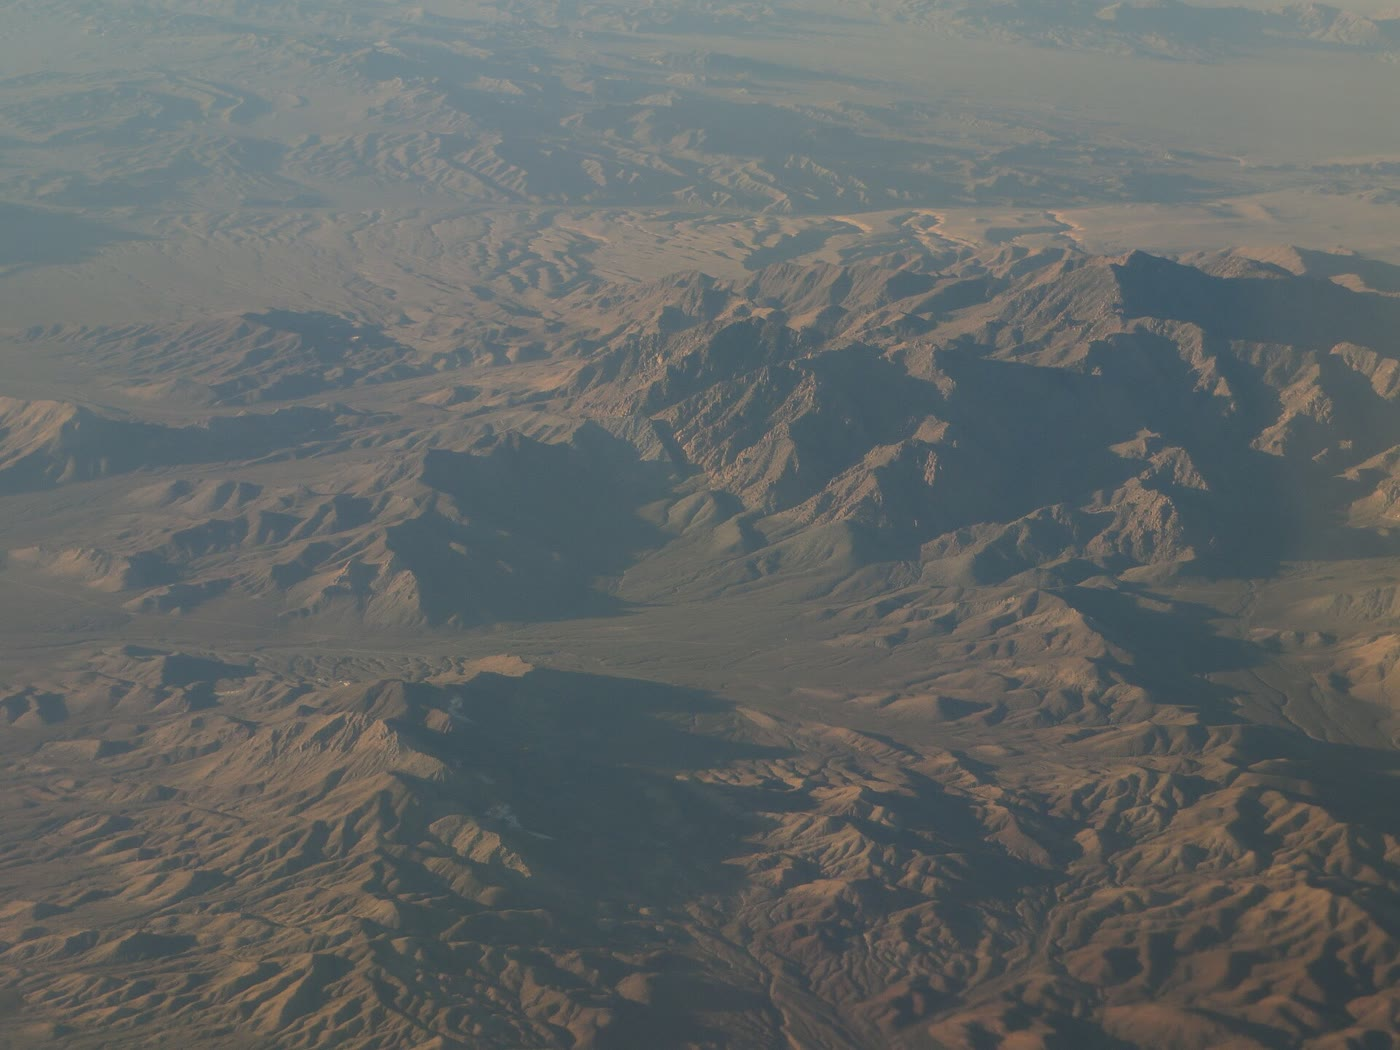
\includegraphics[width=\linewidth]{images/book5/b3-basin-and-range.jpg}

{\scriptsize Basin-and-range topography south of Death Valley, California,
from the air: parallel ranges of tilted fault blocks separated by
sediment-filled basins. Photo Ken Lund, CC BY-SA 2.0.}
\end{minipage}
\end{inthefield}
% ledger: photo:b3-basin-and-range

\section{Exercises}

\begin{exercise}[$\star$]\label{exo:b3:extension-strike-slip:1}
A domain of rigid dominoes has faults that dip \ang{35}; they formed at
\ang{50}. Compute the dip of the beds and the extension factor.
\end{exercise}

\begin{exercise}[$\star$]\label{exo:b3:extension-strike-slip:2}
Say whether each step opens a basin or raises a ridge: a dextral fault
stepping right; a dextral fault stepping left; a sinistral fault stepping
left; a sinistral fault stepping right.
\end{exercise}

\begin{exercise}[$\star$]\label{exo:b3:extension-strike-slip:3}
The Dead Sea Transform has moved \qty{105}{km} in about \qty{20}{Myr}.
Compute the mean rate in \unit{mm/yr} and compare it with the \qty{6}{mm/yr}
used for the Dead Sea basin.
\end{exercise}

\begin{exercise}[$\star$]\label{exo:b3:extension-strike-slip:4}
In the central Basin and Range, \qty{235}{km} of extension amounts to
\qty{200}{\percent}. Compute the width of the region before and after. Do the
same for the northern part, at \qty{50}{\percent}.
\end{exercise}

\begin{exercise}[$\star\star$]\label{exo:b3:extension-strike-slip:5}
The San Andreas fault has moved at least \qty{563}{km} in 15 to
\qty{20}{Myr}. Compute the range of mean rates, and compare them with a
present drift of about \qty{51}{mm/yr}. What could explain the difference?
\end{exercise}

\begin{exercise}[$\star\star$]\label{exo:b3:extension-strike-slip:6}
With $\mu = 0.6$, compute the ratio $\sigma_1/\sigma_3$ needed to slip normal
faults dipping \ang{60}, \ang{50} and \ang{40}, and the lock-up dip.
\end{exercise}

\begin{exercise}[$\star\star$]\label{exo:b3:extension-strike-slip:7}
Compute the lock-up dip of a normal fault for $\mu = 0.4$ and $\mu = 0.2$.
What friction coefficient would let a fault dipping \ang{15} slip under a
vertical $\sigma_1$?
\end{exercise}

\begin{exercise}[$\star\star$]\label{exo:b3:extension-strike-slip:8}
On a seismic section parallel to the slip, a \omterm{def:b3:extension-strike-slip:detachment}{listric fault} has a heave of
\qty{2.5}{km}; it flattens into a detachment \qty{4.0}{km} deep. Compute the
area of the sag below the original top of the hanging wall, and below a bed
first \qty{1.5}{km} deep.
\end{exercise}

\begin{exercise}[$\star\star$]\label{exo:b3:extension-strike-slip:9}
The Dead Sea basin is \qty{132}{km} long and stretched by the factor 1.19
along its axis. Compute its initial length and the stretching, and the time
that stretching takes at \qty{6}{mm/yr}.
\end{exercise}

\begin{exercise}[$\star\star\star$]\label{exo:b3:extension-strike-slip:10}
Blocks \qty{3.0}{km} apart, measured perpendicular to their faults, rotate
from fault dips of \ang{60} to \ang{45}. Compute the horizontal width of one
block before and after, the extension per block, and the dip of the beds.
Why must the beds dip the other way from the faults?
\end{exercise}

\begin{exercise}[$\star\star\star$]\label{exo:b3:extension-strike-slip:11}
Give the angles of the R and R$'$ shears and of the tension fractures for a
rock with $\phi = \ang{40}$ in a sinistral zone striking east--west, as
azimuths, and their senses of slip.
\end{exercise}

\begin{exercise}[$\star\star\star$]\label{exo:b3:extension-strike-slip:12}
A domain of dominoes forms with its faults at the best dip for slip and
rotates until they lock up. Compute the largest extension factor that
rotation alone gives for $\mu = 0.6$ and for $\mu = 0.85$, and say which
rocks can be extended further before new faults must form.
\end{exercise}

\section{Problem: The Merrow Half-Graben}

\begin{problem}[{Weekend problem --- the extension of an invented rift
border, from its dominoes, its listric fault, its core complex and its
transfer fault}]
\label{pb:b3:extension-strike-slip:1}
% values: calc/ch09.py; domino_extension.py; rollover.py
The Merrow half-graben is an invented basin on the border of a continental
rift. Its master fault is listric, dipping \ang{60} at the surface. In its
hanging wall a domain \qty{24.0}{km} wide is cut by planar faults now dipping
\ang{42} east, between which the beds dip \ang{18} west. On a seismic section
parallel to the slip, the master fault has a heave of \qty{3.2}{km} and the
top of its hanging wall sags below its original level over an area of
\qty{16.0}{km^2}. Along strike to the south, erosion has removed the upper
plate of the same system and exposed a core complex. To the north, a
sinistral transfer fault links the half-graben to the next one. Take $\mu =
0.6$, $g = \qty{9.8}{m/s^2}$ and a crustal density of
\qty{2800}{kg/m^3}.

\medskip\noindent\textbf{Part I --- The dominoes.}
\begin{enumerate}
  \item Why is the initial dip of the faults the sum of the present fault and
        bed dips? Give it, and compare it with Anderson's theory.
  \item Compute the extension factor of the domain.
  \item Compute its initial width and the extension it records.
  \item Compute the ratio $\sigma_1/\sigma_3$ needed to slip the faults now,
        and compare it with that of new, well-oriented faults.
  \item At what dip do these faults lock up, and what extension factor could
        the domain reach by rotation alone? What happens then?
\end{enumerate}

\medskip\noindent\textbf{Part II --- The listric master fault.}
\begin{enumerate}[resume]
  \item Explain, with the constant-heave construction, why the hanging-wall
        beds tilt towards the fault.
  \item Compute the depth of the detachment.
  \item The sag area is known to \qty{10}{\percent}. How well is the depth
        known?
  \item What sag area do you predict for a bed that was first \qty{2.0}{km}
        deep?
  \item What is the horizontal extension across the master fault?
  \item How do the sediments of the half-graben record the activity of the
        fault?
\end{enumerate}

\medskip\noindent\textbf{Part III --- The core complex.}
\begin{enumerate}[resume]
  \item Mylonites of the footwall equilibrated at \qty{5.5}{kbar}. Compute
        their depth.
  \item Their micas closed to argon at \qty{24}{Ma}, and pebbles of the same
        mylonites appear in the half-graben fill at \qty{16}{Ma}. Compute the
        mean exhumation rate, taking the closure depth as the depth of the
        previous question.
  \item To bring the mylonites up, how much slip is needed on a detachment
        of mean dip \ang{30}, and how much horizontal extension?
  \item The detachment dips \ang{15} at the surface today. Could it have
        slipped at that dip under a vertical $\sigma_1$? Give two ways out.
  \item If it slipped at \ang{45} at depth, through what angle has the
        exposed part rotated, and why?
  \item Compare the extension of the core complex with that of the
        half-graben.
\end{enumerate}

\medskip\noindent\textbf{Part IV --- The transfer fault.}
\begin{enumerate}[resume]
  \item The sinistral transfer fault steps left by \qty{4.0}{km}, its two
        strands overlapping over \qty{3.0}{km}. Does the step open a basin
        or raise a ridge?
  \item The fault has slipped at \qty{5}{mm/yr} for \qty{1.2}{Myr}. Compute
        the offset.
  \item Compute the area opened, the length of the basin floor (overlap plus
        offset) and its ratio of length to width.
  \item Compare that ratio with the Dead Sea basin's, \qty{132}{km} long and 7
        to \qty{10}{km} wide.
  \item Where the same fault bends the other way, what structure forms, and
        what would a cross-section through it show?
  \item What is the total horizontal extension across the Merrow half-graben,
        from its master fault and its dominoes?
\end{enumerate}
\end{problem}
